%% abtex2-modelo-trabalho-academico.tex, v-1.9.6 laurocesar
%% Copyright 2012-2016 by abnTeX2 group at http://www.abntex.net.br/ 
%%
%% This work may be distributed and/or modified under the
%% conditions of the LaTeX Project Public License, either version 1.3
%% of this license or (at your option) any later version.
%% The latest version of this license is in
%%   http://www.latex-project.org/lppl.txt
%% and version 1.3 or later is part of all distributions of LaTeX
%% version 2005/12/01 or later.
%%
%% This work has the LPPL maintenance status `maintained'.
%% 
%% The Current Maintainer of this work is the abnTeX2 team, led
%% by Lauro César Araujo. Further information are available on 
%% http://www.abntex.net.br/
%%
%% This work consists of the files abntex2-modelo-trabalho-academico.tex,
%% abntex2-modelo-include-comandos and abntex2-modelo-references.bib
%%

% ------------------------------------------------------------------------
% ------------------------------------------------------------------------
% abnTeX2: Modelo de Trabalho Academico (tese de doutorado, dissertacao de
% mestrado e trabalhos monograficos em geral) em conformidade com 
% ABNT NBR 14724:2011: Informacao e documentacao - Trabalhos academicos -
% Apresentacao
% ------------------------------------------------------------------------
% ------------------------------------------------------------------------

\documentclass[
	% -- opções da classe memoir --
	12pt,				% tamanho da fonte
	openright,			% capítulos começam em pág ímpar (insere página vazia caso preciso)
	twoside,			% para impressão em recto e verso. Oposto a oneside
	a4paper,			% tamanho do papel. 
	% -- opções da classe abntex2 --
	%chapter=TITLE,		% títulos de capítulos convertidos em letras maiúsculas
	%section=TITLE,		% títulos de seções convertidos em letras maiúsculas
	%subsection=TITLE,	% títulos de subseções convertidos em letras maiúsculas
	%subsubsection=TITLE,% títulos de subsubseções convertidos em letras maiúsculas
	% -- opções do pacote babel --
	english,			% idioma adicional para hifenização
	french,				% idioma adicional para hifenização
	spanish,			% idioma adicional para hifenização
	brazil				% o último idioma é o principal do documento
	]{abntex2}

% ---
% Pacotes básicos 
% ---
\usepackage{lmodern}			% Usa a fonte Latin Modern			
\usepackage[T1]{fontenc}		% Selecao de codigos de fonte.
\usepackage[utf8]{inputenc}		% Codificacao do documento (conversão automática dos acentos)
\usepackage{lastpage}			% Usado pela Ficha catalográfica
\usepackage{indentfirst}		% Indenta o primeiro parágrafo de cada seção.
\usepackage{color}				% Controle das cores
\usepackage{graphicx}			% Inclusão de gráficos
\usepackage{microtype} 			% para melhorias de justificação
% ---
\usepackage[compact]{titlesec}
\titlespacing{\section}{0pt}{*0}{*0}
\titlespacing{\subsection}{0pt}{*0}{*0}
\titlespacing{\subsubsection}{0pt}{*0}{*0}
		
% ---
% Pacotes adicionais, usados apenas no âmbito do Modelo Canônico do abnteX2
% ---
\usepackage{lipsum}				% para geração de dummy text
% ---

% ---
% Pacotes de citações
% ---
\usepackage[brazilian,hyperpageref]{backref}	 % Paginas com as citações na bibl
\usepackage[alf]{abntex2cite}	% Citações padrão ABNT
\usepackage{cite}
\usepackage{hyperref}
\usepackage{cleveref}

% --- 
% CONFIGURAÇÕES DE PACOTES
% --- 

% ---
% Configurações do pacote backref
% Usado sem a opção hyperpageref de backref
\renewcommand{\backrefpagesname}{Citado na(s) página(s):~}
% Texto padrão antes do número das páginas
\renewcommand{\backref}{}
% Define os textos da citação
\renewcommand*{\backrefalt}[4]{
	\ifcase #1 %
		Nenhuma citação no texto.%
	\or
		Citado na página #2.%
	\else
		Citado #1 vezes nas páginas #2.%
	\fi}%
% ---

% ---
% Informações de dados para CAPA e FOLHA DE ROSTO
% ---
\titulo{Aplicativo móvel para educação ambiental}
\autor{Flávio Telles Paschoal Santos}
\local{Rio das Ostras}
\data{2018}
\orientador{Carlos Bazilio}
\coorientador{Flavio Machado}
\instituicao{%
  UNIVERSIDADE FEDERAL FLUMINENSE
  \par
  PÓLO UNIVERSITÁRIO DE RIO DAS OSTRAS
  \par
   \par
  INSTITUTO DE CIÊNCIA E TECNOLOGIA
  \par
 CURSO DE BACHARELADO EM CIÊNCIA DA COMPUTAÇÃO}
\tipotrabalho{Trabalho de conclusão de curso (Bacharelado)}
% O preambulo deve conter o tipo do trabalho, o objetivo, 
% o nome da instituição e a área de concentração 
\preambulo{}
% ---


% ---
% Configurações de aparência do PDF final

% alterando o aspecto da cor azul
\definecolor{blue}{RGB}{41,5,195}

% informações do PDF
\makeatletter
\hypersetup{
     	%pagebackref=true,
		pdftitle={\@title}, 
		pdfauthor={\@author},
    	pdfsubject={\imprimirpreambulo},
	    pdfcreator={LaTeX with abnTeX2},
		pdfkeywords={abnt}{latex}{abntex}{abntex2}{trabalho acadêmico}, 
		colorlinks=true,       		% false: boxed links; true: colored links
    	linkcolor=blue,          	% color of internal links
    	citecolor=blue,        		% color of links to bibliography
    	filecolor=magenta,      		% color of file links
		urlcolor=blue,
		bookmarksdepth=4
}
\makeatother
% --- 

% --- 
% Espaçamentos entre linhas e parágrafos 
% --- 

% O tamanho do parágrafo é dado por:
\setlength{\parindent}{1.3cm}

% Controle do espaçamento entre um parágrafo e outro:
\setlength{\parskip}{0.2cm}  % tente também \onelineskip

% ---
% compila o indice
% ---
\makeindex
% ---

% ----
% Início do documento
% ----
\begin{document}

% Seleciona o idioma do documento (conforme pacotes do babel)
%\selectlanguage{english}
\selectlanguage{brazil}

% Retira espaço extra obsoleto entre as frases.
\frenchspacing 

% ----------------------------------------------------------
% ELEMENTOS PRÉ-TEXTUAIS
% ----------------------------------------------------------
% \pretextual

% ---
% Capa
% ---
\imprimircapa
% ---

% ---
% Folha de rosto
% (o * indica que haverá a ficha bibliográfica)
% ---
\imprimirfolhaderosto
% ---



% ---
% Inserir folha de aprovação
% ---

% Isto é um exemplo de Folha de aprovação, elemento obrigatório da NBR
% 14724/2011 (seção 4.2.1.3). Você pode utilizar este modelo até a aprovação
% do trabalho. Após isso, substitua todo o conteúdo deste arquivo por uma
% imagem da página assinada pela banca com o comando abaixo:
%
% \includepdf{folhadeaprovacao_final.pdf}
%
\begin{folhadeaprovacao}

  \begin{center}
    {\ABNTEXchapterfont\large\imprimirautor}

    \vspace*{\fill}\vspace*{\fill}
    \begin{center}
      \ABNTEXchapterfont\bfseries\Large\imprimirtitulo
    \end{center}
    \vspace*{\fill}
    
    \hspace{.45\textwidth}
    \begin{minipage}{.5\textwidth}
        \imprimirpreambulo
    \end{minipage}%
    \vspace*{\fill}
   \end{center}
        
   Trabalho aprovado. \imprimirlocal, 15 de dezembro de 2018:

   \assinatura{\textbf{\imprimirorientador} \\ Orientador} 
   \assinatura{\textbf{Professor} \\ Convidado 1}
   \assinatura{\textbf{Professor} \\ Convidado 2}
   %\assinatura{\textbf{Professor} \\ Convidado 3}
   %\assinatura{\textbf{Professor} \\ Convidado 4}
      
   \begin{center}
    \vspace*{0.5cm}
    {\large\imprimirlocal}
    \par
    {\large\imprimirdata}
    \vspace*{1cm}
  \end{center}
  
\end{folhadeaprovacao}
% ---

% ---
% Dedicatória
% ---
\begin{dedicatoria}
   \vspace*{\fill}
   \centering
   \noindent
   \textit{ Este trabalho é dedicado às crianças adultas que,\\
   quando pequenas, sonharam em se tornar cientistas.} \vspace*{\fill}
\end{dedicatoria}
% ---

% ---
% Agradecimentos
% ---
\begin{agradecimentos}


\end{agradecimentos}
% ---




% ---
% RESUMOS
% ---

% resumo em português
\setlength{\absparsep}{18pt} % ajusta o espaçamento dos parágrafos do resumo
\begin{resumo}

 O Brasil produz lixo em quantidades semelhantes à de países desenvolvidos, porem suas políticas e infraestrutura de descarte são equivalentes à de países pobres. A falta de infraestrutura para o recolhimento do lixo é o principal vilão quando se trata de reciclagem, somente 2\% de todo lixo produzido é reciclado.
	Segundo o IBGE em 2015, 77.1\% dos brasileiros possuem um telefone celular e 64.7\% possuem acesso à internet. Logo, o presente trabalho tem como objetivo facilitar o acesso às informações por meio do uso da tecnologia móvel para incentivar aqueles que tem acesso à infraestrutura a descartar corretamente os materiais. Os acessos às informações serão disponibilizados através de um aplicativo que será desenvolvido ao longo desse projeto para que os usuários possam ter um melhor entendimento dos problemas econômicos e sociais causados pelo lixo não reciclado de modo que esses usuários possam desenvolver uma consciência crítica sobre o descarte do lixo doméstico.


 \textbf{Palavras-chave}: Reciclagem, Tecnologia móvel.
\end{resumo}

% resumo em inglês
\begin{resumo}[Abstract]
 \begin{otherlanguage*}{english}
   Brazil produces garbage in quantities similar to those of developed countries, but its policies and disposal infrastructure are equivalent to those of poor countries. The lack of infrastructure for garbage collection is the main villain when it comes to recycling, only 2 \% of all garbage produced is recycled.
According to IBGE in 2015, 77.1 \% of Brazilians have a cell phone and 64.7 \% have access to the internet. Therefore, the present work aims to facilitate access to information through the use of mobile technology to encourage those who have access to the infrastructure to properly discard the materials. Access to information will be made available through an application that will be developed throughout this project so that users can gain a better understanding of the economic and social problems caused by non-recycled litter so that users can develop a critical awareness of the disposal of domestic waste.

   \vspace{\onelineskip}
 
   \noindent 
   \textbf{Keywords}: Recycling, Mobile Technology.
 \end{otherlanguage*}
\end{resumo}



% ---
% inserir lista de ilustrações
% ---
\pdfbookmark[0]{\listfigurename}{lof}
\listoffigures*
\cleardoublepage
% ---

% ---
% inserir lista de tabelas
% ---
\pdfbookmark[0]{\listtablename}{lot}
\listoftables*
\cleardoublepage
% ---

% ---
% inserir lista de abreviaturas e siglas
% ---
\begin{siglas}
  \item[SDK] Software Development Kit  
\end{siglas}
% ---



% ---
% inserir lista de símbolos
% ---
%\begin{simbolos}
%  \item[$ \Gamma $] Letra grega Gama
%  \item[$ \Lambda $] Lambda
%  \item[$ \zeta $] Letra grega minúscula zeta
%  \item[$ \in $] Pertence
%\end{simbolos}
% ---

% ---
% inserir o sumario
% ---


\pdfbookmark[0]{\contentsname}{toc}
\tableofcontents*
\cleardoublepage

% ---



% ----------------------------------------------------------
% ELEMENTOS TEXTUAIS
% ----------------------------------------------------------
\textual

% ----------------------------------------------------------
% Introdução (exemplo de capítulo sem numeração, mas presente no Sumário)
% ----------------------------------------------------------




% ----------------------------------------------------------
% PARTE
% ----------------------------------------------------------
\chapter{Introdução}
% ----------------------------------------------------------
\section{Motivação}
Com o aumento exponencial da população cresce também de forma exponencial o consumo de matéria prima e a quantidade de lixo produzido. Ao longo dos anos surgiram novas maneiras de reaproveitar esses materiais que antes eram descartados em lixões e aterros, como plásticos, papeis, metais e vidros. Muito desses componentes quando não descartados ou tratados de forma adequadas demoram anos e até séculos para de decompor. O acúmulo desses resíduos tem um grande impacto ambiental, destruindo ecossistemas e espécies no seu processo de decomposição. Além disso, o acúmulo desses resíduos tem um grande impacto na saúde e na economia. Os resíduos não descartados de forma correta atuam como facilitadores na disseminação de doenças, o que gera um aumento significativo dos gastos com a saúde. O impacto econômico da reciclagem vai além dos gastos convencionais com a saúde, através dessa prática é possível obter renda extra com produtos reciclados, diminuir a extração de matéria prima tornando os produtos mais baratos e incentivando empreendedores a investir neste ramo e assim gerando mais empregos diretos e indiretos. 
\section{Objetivo}
\subsection{Objetivo Geral}
O objetivo principal desse projeto é o desenvolvimento de um aplicativo mobile (software) nativo para sistemas Android, essa tecnologia permitirá usuários interessados em adquirir novos conhecimentos sobre o processo, composição e impacto dos resíduos produzidos em todo o mundo.

\subsection{Objetivos Específicos}
\begin{itemize}
	\item Este projeto também tem como objetivo entregar conteúdo dinâmico através de um painel administrativo e um serviço web, que será usado para inserir e manter o conteúdo apresentado no aplicativo.
    \item Solucionar problemas de conectividade causados pela mobilidade dos dispositivos, permitindo que o usuário acesse o conteúdo quando estiver sem acesso à internet.
        \item Solucionar problemas relacionados a dimensão de telas e garantir a retro compatibilidade com dispositivos mais antigos.
\end{itemize}
% ---

% ----------------------------------------------------------
\chapter{Trabalhos relacionados}
% ----------------------------------------------------------

Nesta sessão serão apresentados três trabalhados, dois aplicativos móveis e uma pagina da internet que possuem funcionalidades similares ao projeto atual descrito nesse documento. Funcionalidades não relevantes não serão apresentadas.

\section{Cataki}
O aplicativo atua conectando os catadores com qualquer um que tenha resíduos ou material reciclável a ser recolhido. A ideia é reconhecer o pequeno empreendedorismo ambiental desempenhado por estes profissionais e colaborar com o descarte adequado dos resíduos.

Para utilizar o aplicativo basta efetuar a transferência na Google Play\cite{googleplay} ou na App Store\cite{appstore} e começar a utiliza-lo, o Cataki permite o uso dos seus recursos de forma anônima, facilitando o acesso rápido as suas funcionalidades. É possível também, ainda de forma anônima, cadastrar um novo catador dando visibilidade aos indivíduos que tem dificuldade em manipular recursos de um aplicativo móvel, ou não possuem acesso à internet.

Na \autoref{fig:figura1} pode-se observar a funcionalidade principal do aplicativo, onde um mapa mostrando ícones nas localizações dos catadores, centros de coleta e cooperativas é exibido na tela possibilitando a interação do usuário com esses pontos. Caso um ícone seja selecionado, as informações referente a este fica disponível. A \autoref{fig:figura2} mostra a tela exibida após o ícone do catador ser selecionado, informações como o resíduo que esse catador trabalha e dados relevantes para o contato fica disponível. \\
    

    \begin{figure}[htb]    
 \centering
  \begin{minipage}{0.45\textwidth}
    \centering
    \caption{Cataki - Localizar}
    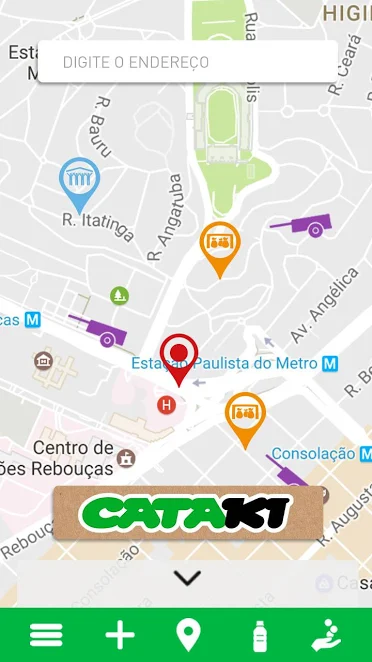
\includegraphics[scale=0.45]{media/catakimap.png}
    \legend{Fonte: Google Play}
     \label{fig:figura1}
  \end{minipage}
  \hfill
  \begin{minipage}{0.45\textwidth}
    \centering
    \caption{Cataki - Catador}
    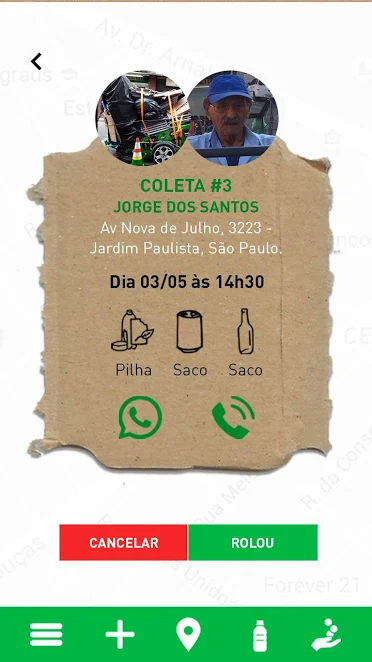
\includegraphics[scale=0.45]{media/infocatador.png}
    \legend{Fonte: Google Play}
     \label{fig:figura2}
  \end{minipage}
\end{figure}

\newpage
O Cataki também possui um banco de dados com informações genéricas sobre o descarte e sobre os materiais. A \autoref{fig:figura3} mostra os materiais disponíveis no aplicativo, quando uma material é selecionado, uma nova tela se abre mostrando os detalhes sobre o mesmo, como mostrado na \autoref{fig:figura4}. \\
     \begin{figure}[htb]    
 \centering
  \begin{minipage}{0.45\textwidth}
    \centering
    \caption{Cataki - Materiais}
    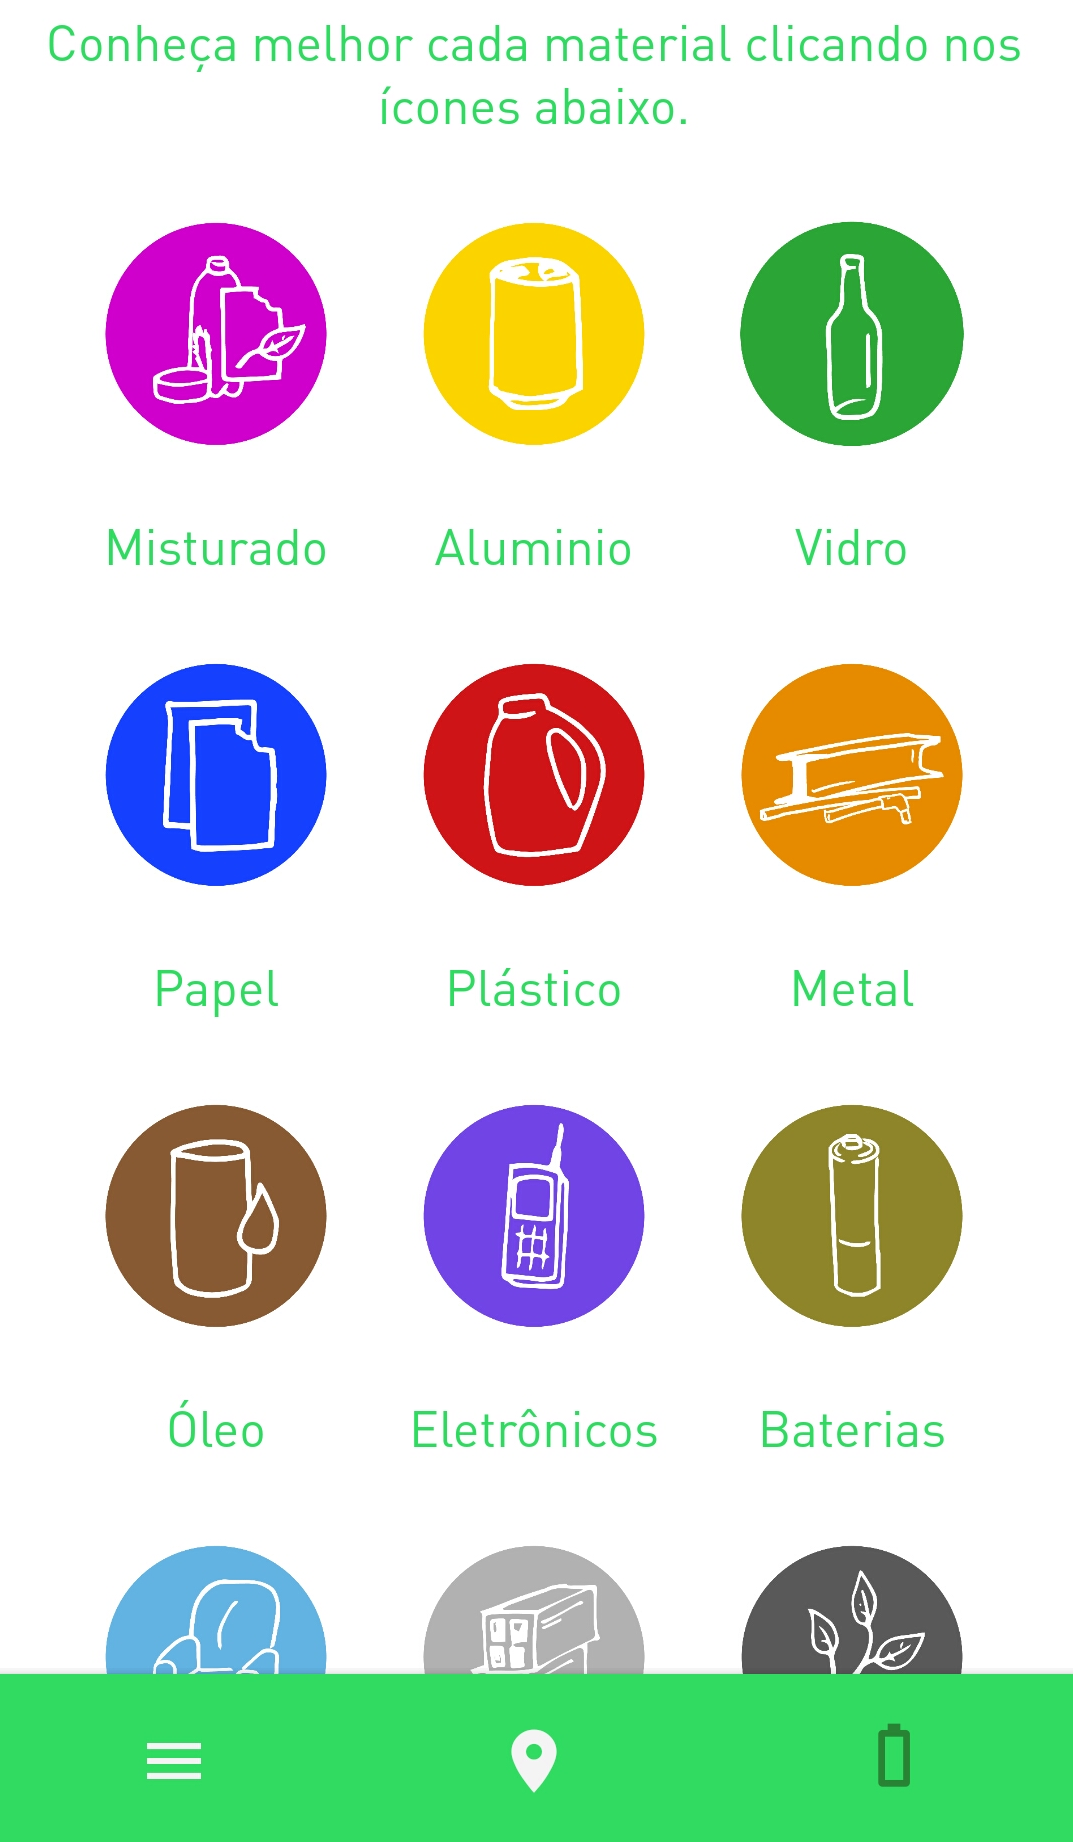
\includegraphics[scale=0.15]{media/catakimateriais.png}   
    \legend{Fonte: Google Play}
     \label{fig:figura3}
  \end{minipage}
  \hfill
  \begin{minipage}{0.45\textwidth}
    \centering
    \caption{Cataki - Detalhes}
    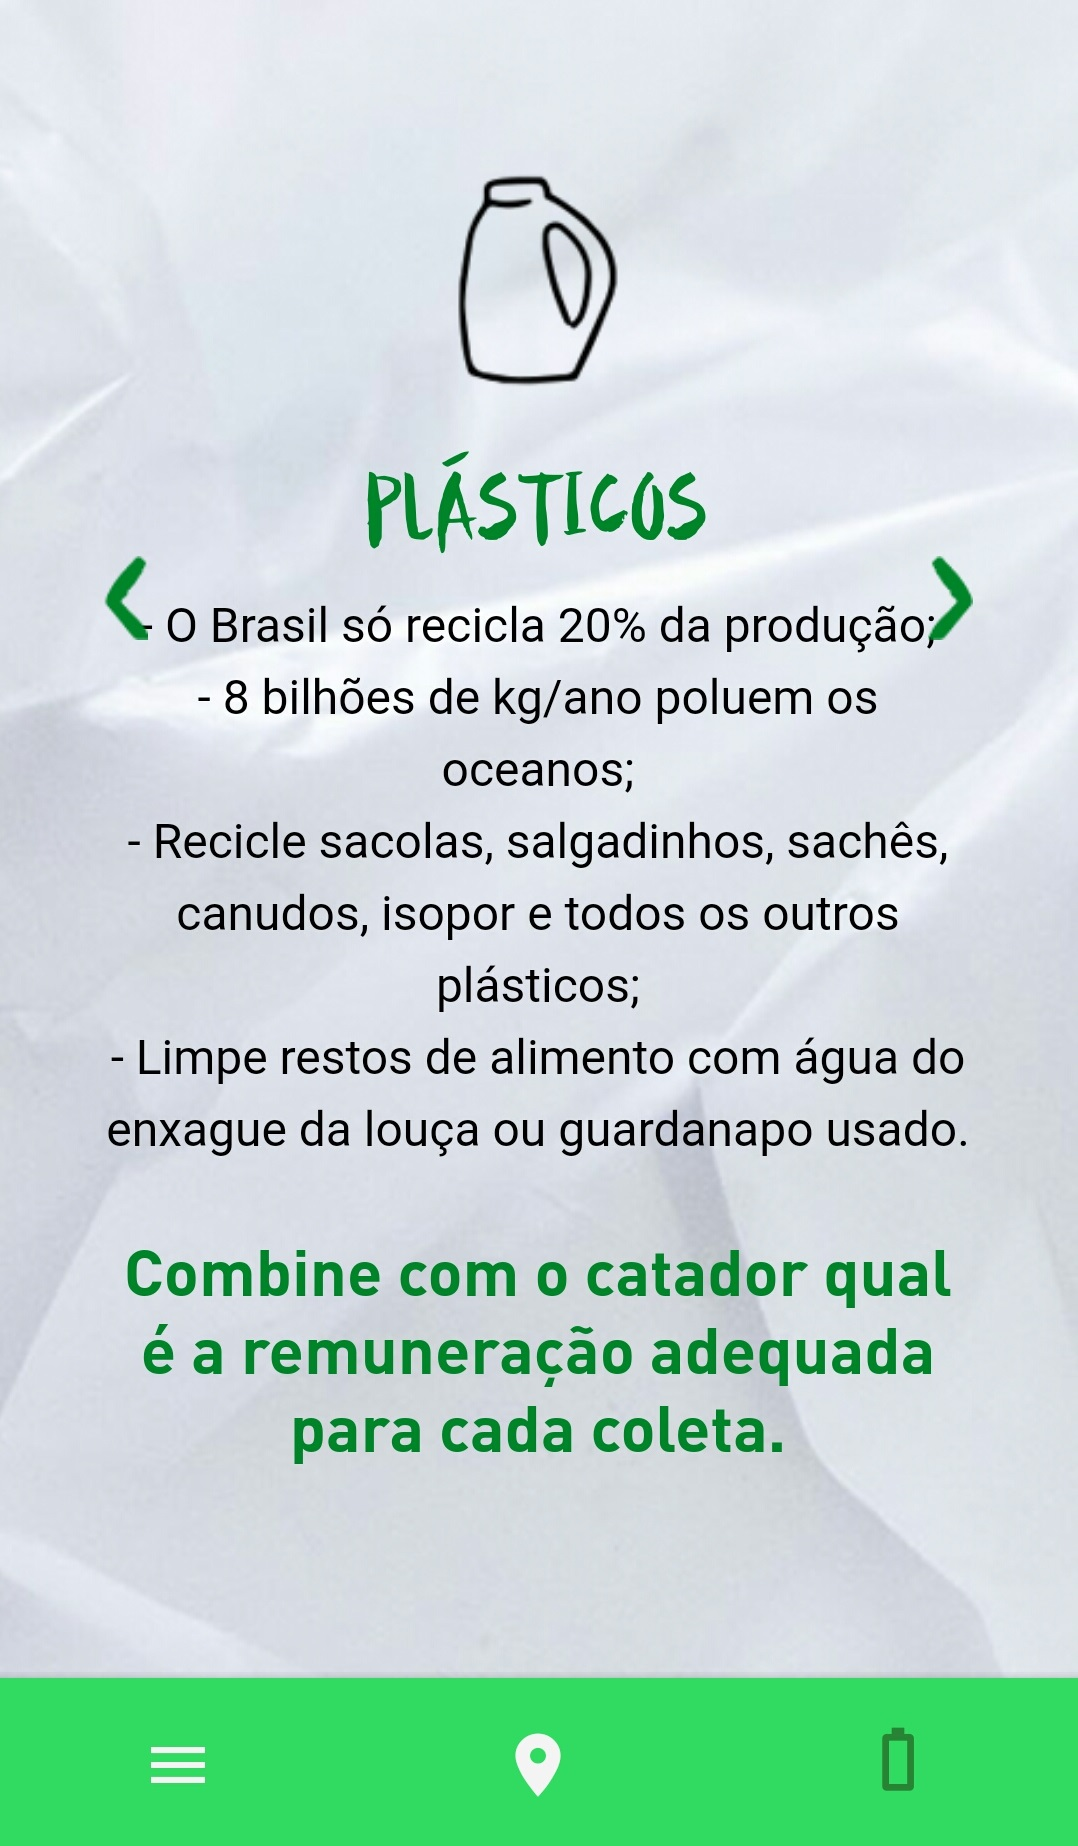
\includegraphics[scale=0.15]{media/catakimateriaisdetalhes.jpg}
    \legend{Fonte: Google Play}
     \label{fig:figura4}
  \end{minipage}
\end{figure}

\section{Recicloteca}

A Recicloteca é um Centro de Informações sobre Reciclagem e Meio Ambiente criado pela ONG Ecomarapendi. Foi desenvolvido com o objetivo de difundir informações sobre as questões ambientais, com ênfase na redução, reaproveitamento e reciclagem de resíduos. Seu acervo é composto pelos mais diversos materiais incluindo livros, vídeos, revistas, periódicos técnico-científicos, cartilhas, teses, produtos reciclados e outros.

Para utilizar a Recicloteca é preciso acessar a pagina na internet \href{http://www.recicloteca.org.br/}{<www.recicloteca.org.br>}, ao acessar a página uma das sessões relevantes para esse trabalho é a sessão de \href{http://www.recicloteca.org.br/pesquisa/}{Pesquisa Escolar} que aparece na página principal, como mostrado na \autoref{fig:reciclotecahome}.

\begin{figure}[h]
\centering
   \caption{Recicloteca - Página Inicial}
   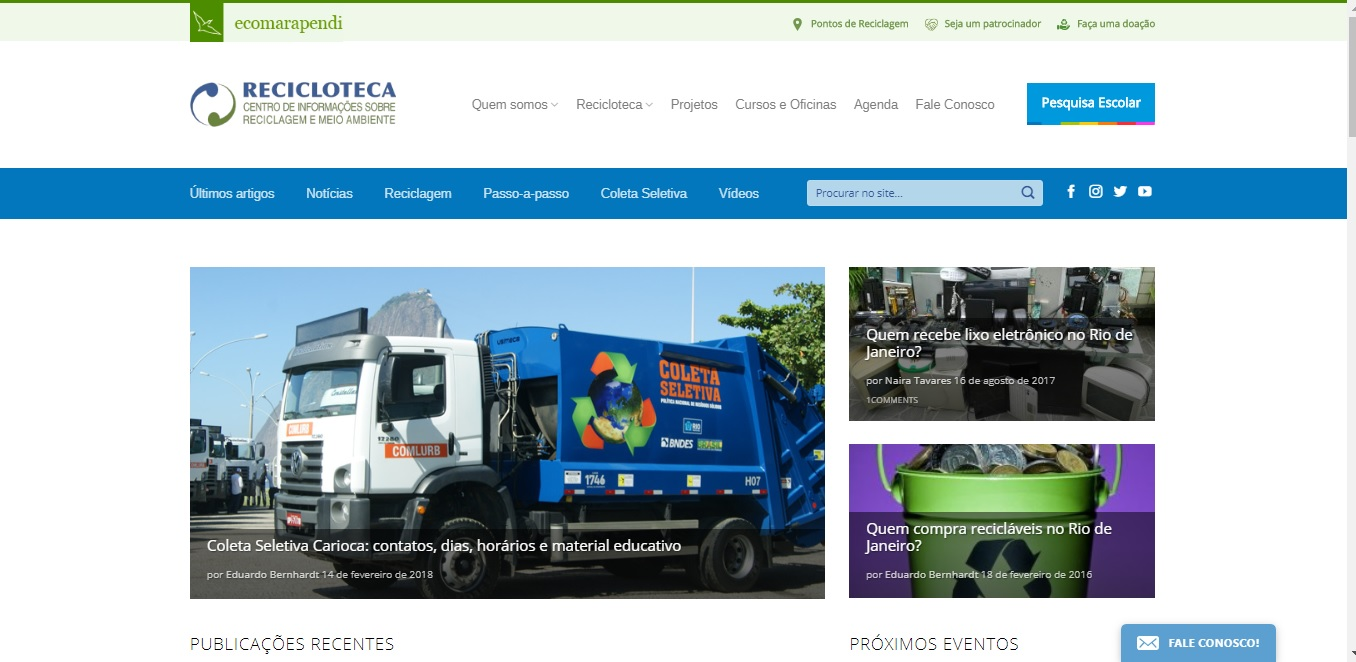
\includegraphics[scale=0.45]{media/reciclotecahome.jpg}
   \legend{Fonte: Recicloteca.org.br}
     \label{fig:reciclotecahome}
\end{figure}

\newpage
Ao clicar em pesquisa escolar, o usuário é redirecionado para uma pagina que contem uma série de vídeos animados separados por diversas categorias, como mostra a \autoref{fig:reciclotecaescola}, esses vídeos são feitos com uma linguagem fácil e uma animação que mantêm o interesse das crianças.


\begin{figure}[h]
\centering
   \caption{Recicloteca - Pesquisa Escolar}
   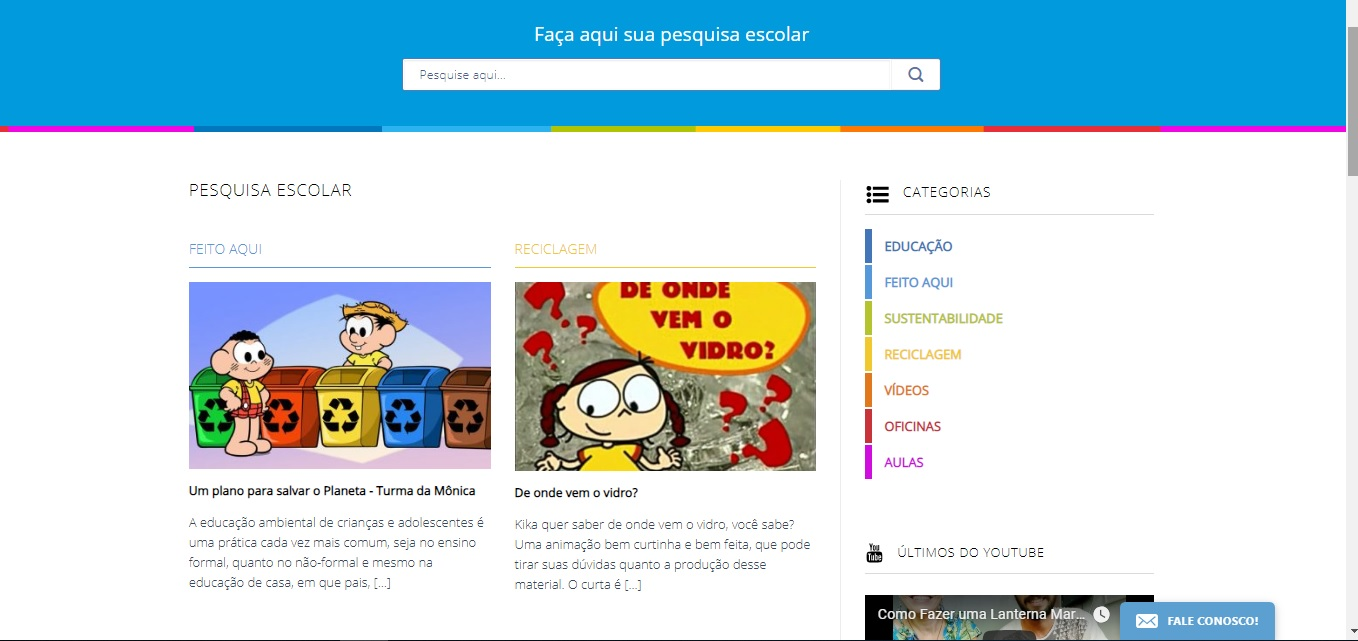
\includegraphics[scale=0.45]{media/reciclotecaescola.jpg}
   \legend{Fonte: Recicloteca.org.br}
     \label{fig:reciclotecaescola}
\end{figure}

\newpage
Outra sessão relevante para esse projeto é a "Passo-a-passo" que pode ser acessada no menu da página principal como mostra a \autoref{fig:reciclotecareciclagem}. Esta sessão contem vídeos e artigos ensinando como reaproveitar itens que seriam descartados dando origem a um novo produto ou a uma nova matéria-prima com o objetivo de diminuir a produção de rejeitos e o seu acúmulo na natureza, reduzindo o impacto ambiental.


\begin{figure}[h]
\centering
   \caption{Recicloteca - Passo-a-passo}
   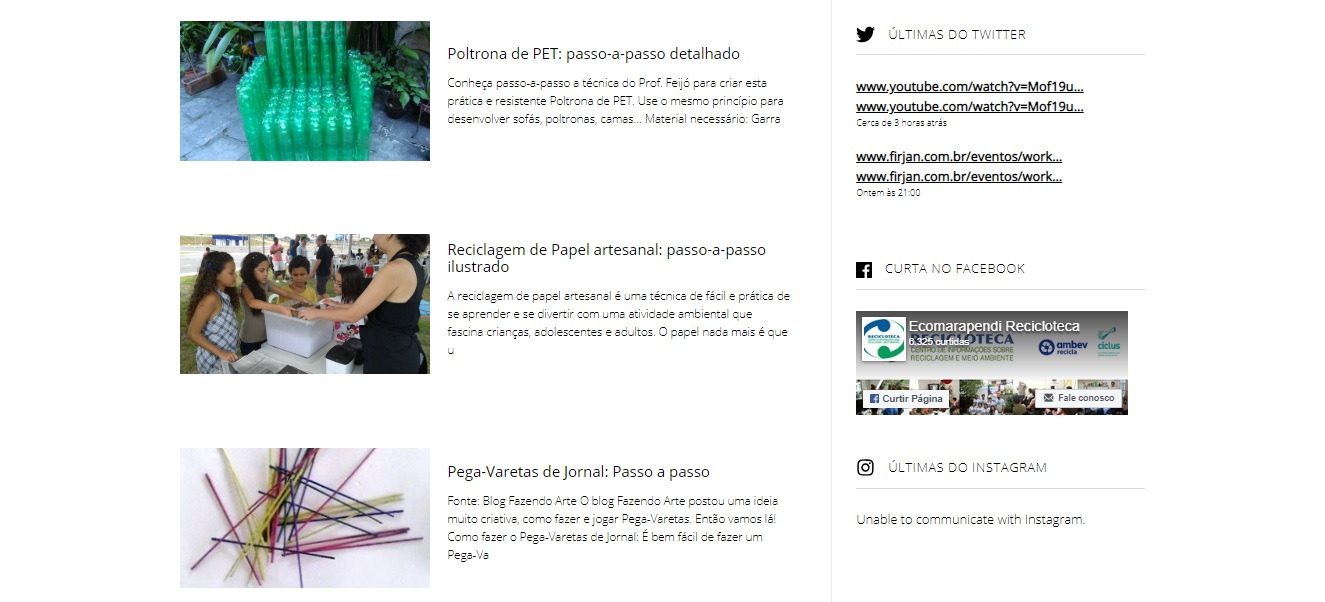
\includegraphics[scale=0.45]{media/reciclotecareciclagem.jpg}
   \legend{Fonte: Recicloteca.org.br}
     \label{fig:reciclotecareciclagem}
\end{figure}


% ---

\newpage
\section{Rota da Reciclagem}

O Rota da Reciclagem é um aplicativo que promove a reciclagem e a defesa do meio ambiente. Este mostra como qualquer pessoa interessada pode participar da separação e entrega das embalagens longa vida para a reciclagem, informando ainda onde estão localizadas as cooperativas de catadores, as empresas comerciais que trabalham com compra de materiais recicláveis e os pontos de entrega voluntária que recebem embalagens da Tetra Pak\cite{tetrapark}.

Para utilizar o aplicativo é preciso efetuar a transferência na Google Play\cite{googleplay} ou na App Store\cite{appstore}, após a transferência basta abrir o aplicativo que apresentará a tela de carregamento. Após o carregamento dos dados uma tela com um campo de texto para inserir o endereço da sua localização aparecerá e ao ser preenchido exibira um mapa mostrando marcadores que representam cooperativas,pontos de entrega, comércios e sua localização atual, como mostra a \autoref{fig:rota2}.
    
    

    
         \begin{figure}[htb]    
 \centering
  \begin{minipage}{0.45\textwidth}
    \centering
    \caption{Rota da reciclagem - Tela de carregamento}
    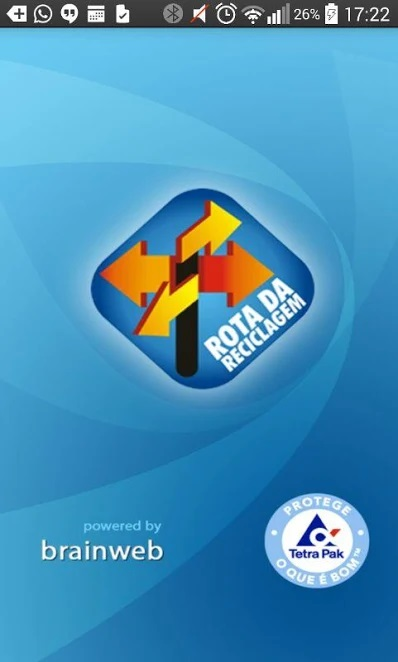
\includegraphics[scale=0.45]{media/rotaappintro.jpg}   
    \legend{Fonte: Google Play}
     \label{fig:rota1}
  \end{minipage}
  \hfill
  \begin{minipage}{0.45\textwidth}
    \centering
    \caption{Rota da reciclagem - Mapa}
    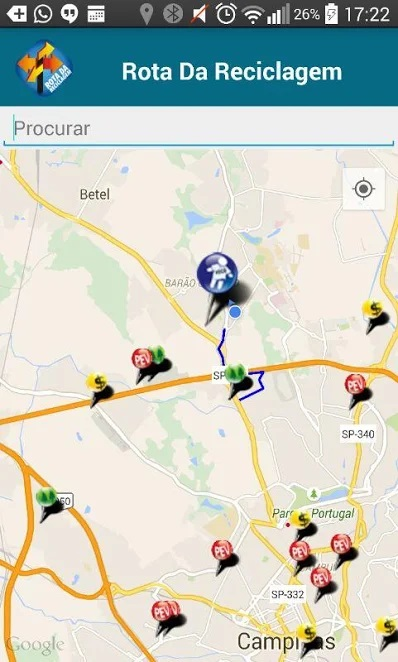
\includegraphics[scale=0.45]{media/rotaappmap.jpg}
    \legend{Fonte: Google Play}
     \label{fig:rota2}
  \end{minipage}
\end{figure}




% ----------------------------------------------------------
\begin{chapter}{Projeto}
% ----------------------------------------------------------

Nesta sessão serão apresentadas as principais características referentes ao sistema operacional Android e ao desenvolvimento de aplicativos mobile.

\section{Android O.S}
O Google em parceria com outras empresas lançou o desafio de criar um plataforma móvel em que todos os participantes da aliança pudessem utilizar em seus hardwares e que fosse de acesso economicamente viável à população tirando o peso do custo de desenvolvimento de um sistema móvel completo como é, assim nasceu o Android. Uma pilha de softwares para dispositivos móveis que inclui um sistema operacional, um middleware e um conjunto de aplicações chaves. Os desenvolvedores podem criar aplicações para a plataforma usando o Android SDK (Software Development Kit), uma IDE (Integrated Development Environment) e uma linguagem suportada pela SDK. As aplicações para essa plataforma são comumente escritas usando a linguagem de programação Java ou Kotlin.

Os aplicativos gerados são executados sobre o Dalvik, uma máquina virtual customizada para dispositivos com restrições de recursos, como pouca capacidade computacional, baixa capacidade de armazenamento e baterias com baixo nível de energia.

\newpage
\subsection{Arquitetura}
A arquitetura do sistema operacional Android é divida em camadas, onde cada camada é responsável por gerenciar os seus processos. O diagrama na \autoref{fig:arquitetura} mostra essa divisão.

\begin{figure}[h]
\centering
   \caption{Arquitetura Android}
   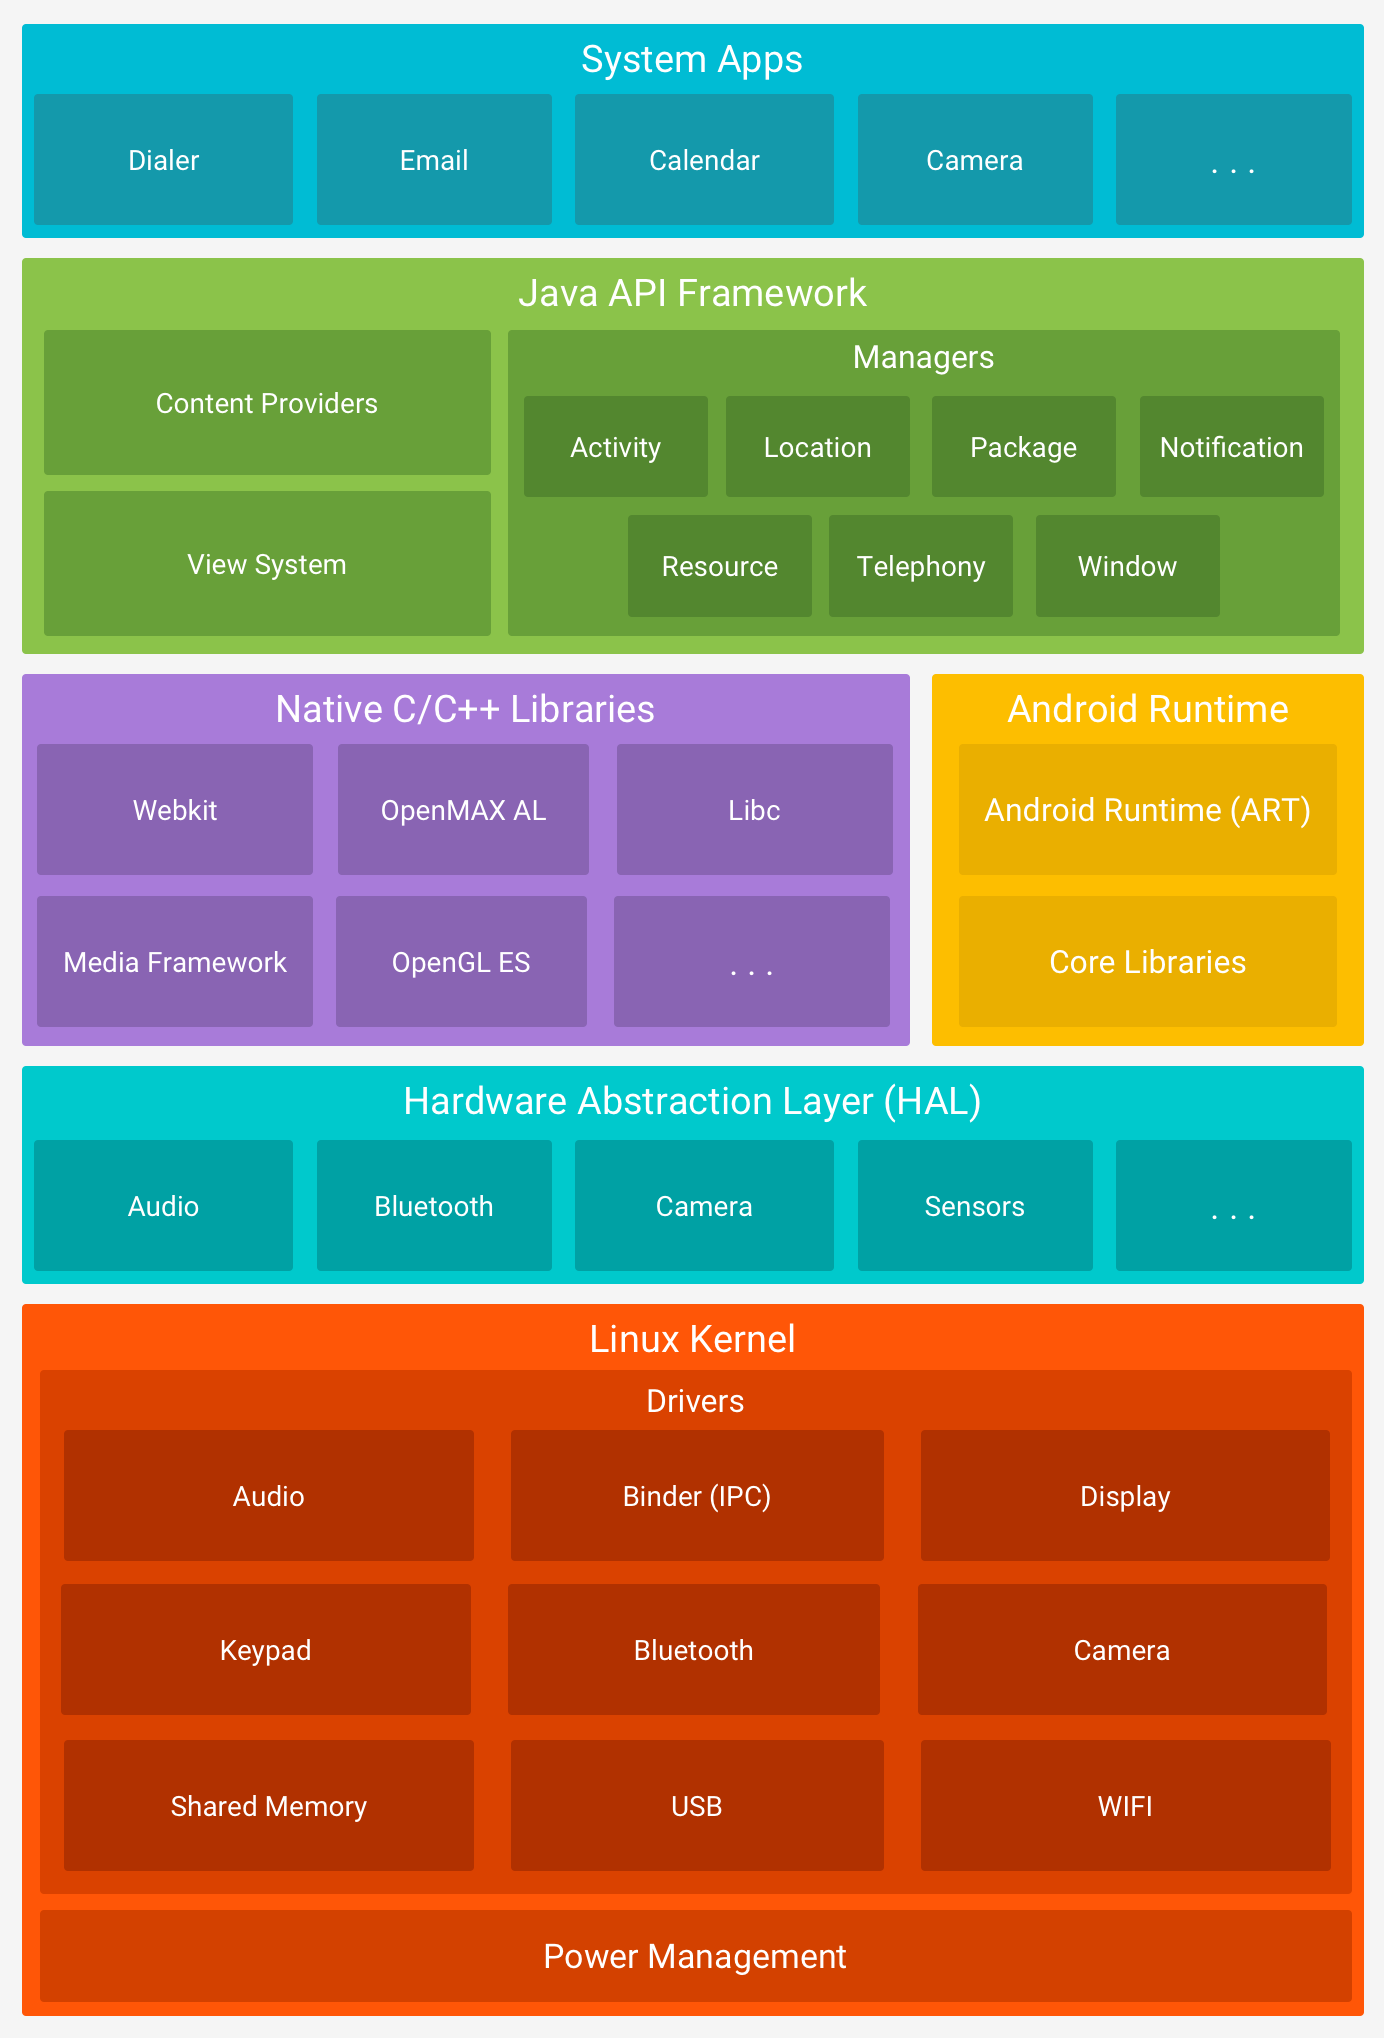
\includegraphics[scale=0.20]{media/android-stack_2x.png}
   \legend{Fonte: developer.android.com}
     \label{fig:arquitetura}
\end{figure}


\subsubsection{Kernel}
Os dispositivos móveis possuem arquiteturas distintas e para isso é necessária uma camada capaz de gerenciar os recursos do sistema, além de fornecer aos programas do usuário uma interface simplificada com o hardware.
O sistema operacional Android utiliza o kernel do Linux, que é responsável por gerenciar serviços como segurança, gerenciamento de memória, processos, rede e drivers.


\subsubsection{Android Runtime}
O Android Runtime (ART) é um processo responsável pela compilação de códigos de alto nivel (DEX bytecode) em codigos de maquina.
O processo usa uma técnica de compilação chamada AOT (Ahead of Time), sua principal diferença em relação ao Dalvik é que ela ocorre antes 
da execução do aplicativo e não durante a execução. Com isso, há um aumento na velocidade de execução ao custo de um processo que ocupa mais memoria.

\subsubsection{Native C/C++ Libraries}
Vários componentes e diversos serviços do sistema operacional Android são implementados em código nativo,
 o que exige bibliotecas nativas desenvolvidas em C e C++.
O framework Android oferece uma camada de abstração chamada de HAL (Hardware abstraction layer) para expor as funcionalidades de algumas dessas bibliotecas,
 tal abstração permite a manipulação de vídeos, imagens, sons, animações, GPS, etc.



\subsection{Máquina Virtual}
O Lorem Ipsum é um texto modelo da indústria tipográfica e de impressão. O Lorem Ipsum tem vindo a ser o texto padrão usado por estas indústrias desde o ano de 1500, quando uma misturou os caracteres de um texto para criar um espécime de livro. Este texto não só sobreviveu 5 séculos, mas também o salto para a tipografia electrónica, mantendo-se essencialmente inalterada. Foi popularizada nos anos 60 com a disponibilização das folhas de Letraset, que continham passagens com Lorem Ipsum, e mais recentemente com os programas de publicação como o Aldus PageMaker que incluem versões do Lorem Ipsum.



\subsection{Aplicação Android}
O Lorem Ipsum é um texto modelo da indústria tipográfica e de impressão. O Lorem Ipsum tem vindo a ser o texto padrão usado por estas indústrias desde o ano de 1500, quando uma misturou os caracteres de um texto para criar um espécime de livro. Este texto não só sobreviveu 5 séculos, mas também o salto para a tipografia electrónica, mantendo-se essencialmente inalterada. Foi popularizada nos anos 60 com a disponibilização das folhas de Letraset, que continham passagens com Lorem Ipsum, e mais recentemente com os programas de publicação como o Aldus PageMaker que incluem versões do Lorem Ipsum.

\subsection{Android SDK}
O Lorem Ipsum é um texto modelo da indústria tipográfica e de impressão. O Lorem Ipsum tem vindo a ser o texto padrão usado por estas indústrias desde o ano de 1500, quando uma misturou os caracteres de um texto para criar um espécime de livro. Este texto não só sobreviveu 5 séculos, mas também o salto para a tipografia electrónica, mantendo-se essencialmente inalterada. Foi popularizada nos anos 60 com a disponibilização das folhas de Letraset, que continham passagens com Lorem Ipsum, e mais recentemente com os programas de publicação como o Aldus PageMaker que incluem versões do Lorem Ipsum.





\newpage
\section{Ambiente de desenvolvimento}
\subsection{Instalação}
\subsection{Configuração}
\section{Ambiente de desenvolvimento}
\section{Modelagem dos dados}
\section{Desenvolvimento do aplicativo}
\end{chapter}
% ----------------------------------------------------------
\chapter{Conclusão}
% ----------------------------------------------------------
\chapter{Trabalhos futuros}



% ----------------------------------------------------------
% ELEMENTOS PÓS-TEXTUAIS
% ----------------------------------------------------------
\postextual
% ----------------------------------------------------------

% ----------------------------------------------------------
% Referências bibliográficas
% ----------------------------------------------------------

\bibliographystyle{alpha}
\bibliography{bibliography.bib}




% ----------------------------------------------------------
% Glossário
% ----------------------------------------------------------
%
% Consulte o manual da classe abntex2 para orientações sobre o glossário.
%
%\glossary

% ----------------------------------------------------------
% Apêndices
% ----------------------------------------------------------





%---------------------------------------------------------------------
% INDICE REMISSIVO
%---------------------------------------------------------------------
\phantompart
\printindex
%---------------------------------------------------------------------

\end{document}
